\documentclass[a4paper]{article} 
\addtolength{\hoffset}{-2.25cm}
\addtolength{\textwidth}{4.5cm}
\addtolength{\voffset}{-3.25cm}
\addtolength{\textheight}{5cm}
\setlength{\parskip}{0pt}
\setlength{\parindent}{0in}

%----------------------------------------------------------------------------------------
%	PACKAGES AND OTHER DOCUMENT CONFIGURATIONS
%----------------------------------------------------------------------------------------

\usepackage{blindtext} % Package to generate dummy text
\usepackage{charter} % Use the Charter font
\usepackage[shortlabels]{enumitem} %for enum purpose
\usepackage[utf8]{inputenc} % Use UTF-8 encoding
\usepackage{microtype} % Slightly tweak font spacing for aesthetics
\usepackage[english]{babel} % Language hyphenation and typographical rules
\usepackage{amsthm, amsmath, amssymb} % Mathematical typesetting
\usepackage{float} % Improved interface for floating objects
\usepackage[final, colorlinks = true, 
            linkcolor = black, 
            citecolor = black]{hyperref} % For hyperlinks in the PDF
\usepackage{graphicx, multicol} % Enhanced support for graphics
\usepackage{xcolor} % Driver-independent color extensions
\usepackage{marvosym, wasysym} % More symbols
\usepackage{rotating} % Rotation tools
\usepackage{censor} % Facilities for controlling restricted text
\usepackage{listings, style/lstlisting} % Environment for non-formatted code, !uses style file!
\usepackage{pseudocode} % Environment for specifying algorithms in a natural way
\usepackage{style/avm} % Environment for f-structures, !uses style file!
\usepackage{booktabs} % Enhances quality of tables
\usepackage{tikz-qtree} % Easy tree drawing tool


\tikzset{every tree node/.style={align=center,anchor=north},
         level distance=2cm} % Configuration for q-trees
\usepackage{style/btree} % Configuration for b-trees and b+-trees, !uses style file!
\usepackage[backend=biber,style=numeric,
            sorting=nyt]{biblatex} % Complete reimplementation of bibliographic facilities
\addbibresource{ecl.bib}
\usepackage{csquotes} % Context sensitive quotation facilities

\newcommand{\note}[1]{\marginpar{\scriptsize \textcolor{red}{#1}}} % Enables comments in red on margin
\usepackage{hyperref}
\hypersetup{
    colorlinks=true,
    linkcolor=blue,
    filecolor=magenta,      
    urlcolor=black,
    }
%----------------------------------------------------------------------------------------

\usepackage{algorithm}
\usepackage{verbatim}
\usepackage[noend]{algpseudocode}
\newcommand{\algrule}[1][.2pt]{\par\vskip.5\baselineskip\hrule height #1\par\vskip.5\baselineskip}
\newcommand{\floor}[1]{\left\lfloor #1 \right\rfloor}
\newcommand{\ceil}[1]{\left\lceil #1 \right\rceil}

\begin{document}

%-------------------------------
%	TITLE SECTION
%-------------------------------

\title{\textbf{COL351 : Analysis and Design of Algorithm \\ Assignment 3 }}
\author{Gaurav Jain (2019CS10349) \& T Abishek (2019CS10407)}
\date{}

%-------------------------------
%	CONTENTS
%-------------------------------

\maketitle

\section{Convex Hull}
The Divide and Conquer algorithm to compute Convex Hull is present below:

{\centering
\begin{minipage}{\linewidth}
\begin{algorithm}[H]
\caption{Convex Hull Algorithm}\label{alg:chull}
\begin{algorithmic}[1]
\Procedure{ConvexHull}{P = \{($x_1$,$y_1$),($x_2$,$y_2$)....($x_n$,$y_n$)\}}
\If{n $\leq$ 5} 
 \State Solve using Brute Force method
\EndIf
\State Sort P in increasing order according to x coordinate
\State Divide P into A and B such that: A contains the left $\floor{\frac{n}{2}}$ points and B contains the right $\ceil{\frac{n}{2}}$ points.

\State $Q_1 \gets$ \textsc{ConvexHull}(A)
\State $Q_2 \gets$ \textsc{ConvexHull}(B)

\State $Q \gets$ \textsc{Merge}($Q_1$,$Q_2$)

\State \Return $Q$

\EndProcedure
\algrule
\Procedure{Merge}{A,B}
\State $(x_1,y_1) \gets$  \textsc{UpperTangent}(A,B)
\State $(x_2,y_2) \gets$ \textsc{LowerTangent}(A,B)
\State U $\gets$ \{\}
\State $u \gets x_1$
\While{$u \neq x_2$}
    \State Add $u$ to U 
    \State $u \gets$ next element in A in counter clockwise direction
\EndWhile
\State $u \gets y_1$
\While{$u \neq y_2$}
    \State Add $u$ to U 
    \State $u \gets$ next element in B in clockwise direction
\EndWhile

\State \Return U
\EndProcedure

\algrule
\Procedure{UpperTangent}{A,B}
\State a $\gets$ Rightmost point of A
\State b $\gets$ Leftmost point of B
\State T $\gets$ (a,b)
\While{T = ab not a tangent to both A and B}
    \While{T not a tangent to A}
    \State a $\gets$ next element in A in counter clockwise direction
    \EndWhile
    
    \While{T not a tangent to B}
    \State b $\gets$ next element in B in clockwise direction
    \EndWhile
\EndWhile

\State \Return T
\EndProcedure
\algrule
\Procedure{LowerTangent}{A,B}
\State a $\gets$ Index of rightmost point of A 
\State b $\gets$ Index of leftmost point of B
\State T $\gets$ ab
\While{T = ab not a tangent to both A and B}
    \While{T not a tangent to A}
    \State a $\gets$ next element in A in clockwise direction
    \EndWhile
    
    \While{T not a tangent to B}
    \State b $\gets$ next element in B in counter clockwise direction
    \EndWhile
\EndWhile

\State \Return T
\EndProcedure

\end{algorithmic}
\end{algorithm}
\end{minipage}
\par}

\newpage
\textbf{Runtime Analysis:}\\

The time complexity of the divide and conquer algorithm to compute convex hull is calculated using the recurrence relation: T(n) = 2T(n/2)+O(n)+merge operation time complexity. Median is calculated in O(n) using $k^{th}$ smallest element problem discussed in lectures. The brute force method is used for base case when $n\leq5$ which take $O(n^3)$ time for n points. Thus, there is only a small increase in runtime.\\ 
The time taken in merge operation depends on the time taken to calculate upper tangent and lower tangent of the two convex hulls to be merged and the time taken to merge these two convex hulls and the two tangents which is performed in a while loop iterating over all elements of A and B.\\
The lower tangent and upper tangent function has same time complexity which is $O(size A)$ for convex hull A. Thus, the time complexity of merge operation is $O(size A)$ + $O(size B)$ + $O(n)$ = $O(n)$.\\

\textbf{Correctness of Algorithm:}\\

\textit{\underline{Claim 1}} \\
The line given by the \textsc{LowerTangent} procedure touches A and B at their lower halves and does not intersect A and B at any other points.\\
\textit{\underline{Proof}} \\
The procedure tends to move both points located on A and B in the same direction and this leads to a line segment which passes through the lowest end of the lower halves of A and B.\\
Due to this movement, line T becomes a direct tangent to the convex hulls A and B. This line also never intersect at any other point of A and B.{\hfill\qed}

\textit{\underline{Claim 2}} \\
The polygon formed after the merging step of two convex hulls A and B is a convex hull.\\
\textit{\underline{Proof}} Proof by Contradiction \\
Since A and B are convex and they are connected using upper and lower tangents, the merged polygon is also convex in nature. Suppose the polygon formed after merging A and B is not a convex hull. This means that there is at least one extra point in the merged polygon.\\
So after removing this point, the new polygon is a convex hull and the removed point should lie inside the new polygon. This implies that the removed point was part of a concave edge which is a contradiction as A and B are convex in nature.
So the above claim holds.{\hfill\qed}\\\\
We can proof the correctness of the algorithm using induction on number of points present in the plane. By dividing the plane into smaller and smaller parts, we reach the base case which is solved using brute force method. Using claim 1 and 2, merging the smaller convex hulls results in the final answer.


\newpage

\section{Particle Interaction}

\textbf{Observation}:\\

F\textsubscript{j} $=$ C q\textsubscript{j} \bigg( $\sum\limits_{i<j}^{}\frac{q\textsubscript{i}}{(j-i)\textsuperscript{2}}$ $-$ $\sum\limits_{i>j}^{}\frac{q\textsubscript{i}}{(j-i)\textsuperscript{2}}$ \bigg)
\\
F\textsubscript{j} $=$ C q\textsubscript{j} c\textsubscript{j}
\\\\

Where, \\
c\textsubscript{k} $=$  $\sum\limits_{i<j}^{}\frac{q\textsubscript{i}}{(j-i)\textsuperscript{2}}$ $-$ $\sum\limits_{i>j}^{}\frac{q\textsubscript{i}}{(j-i)\textsuperscript{2}}$  for all k $\in$ [1,n] \hfill(1)   
\\\\

Consider the two polynomials, \\
A(x) $=$ q\textsubscript{1}x + q\textsubscript{2}x\textsuperscript{2} + . . . + q\textsubscript{n}x\textsuperscript{n}\\

B(x) $=$ $ - \frac{1}{(n-1)\textsuperscript{2}}x -  . . . - \frac{1}{4}x\textsuperscript{n-2} - x\textsuperscript{n-1} - 0$.$x\textsuperscript{n} + x\textsuperscript{n+1} + \frac{1}{4}x\textsuperscript{n+2} + . . . +  \frac{1}{(n-1)\textsuperscript{2}}x\textsuperscript{2n-1} $
\\

Consider the product, P(x) = A(x)$*$B(x). 
\\Co-efficient of x\textsuperscript{k} for k in range (n,2n+1) $=$ $\sum\limits_{l = 1}^n a\textsubscript{l}$b\textsubscript{k-l} \hfill(2)\\\\

From equation (1) and equation (2), it is observable that coefficient of $x^{n+j}$ in P(x) = $c_j$. So, to obtain $c_j$, we need P(x) which can be calculated using Fast Fourier Transform discussed in the lectures. The time complexity here is $O(nlogn)$.
\\\\
Now, using c\textsubscript{j} and equation (1), we can obtain F\textsubscript{j} for all the particles $(j \in [1,n])$ within $O(nlogn)$ time complexity.
\\


{\centering
\begin{minipage}{\linewidth}
\begin{algorithm}[H]
\caption{Particle Interaction Algorithm}\label{pia}
\begin{algorithmic}[1]
\Procedure{ParticleInteraction}{}
\State{$A$ $\gets$ $[q\textsubscript{1}, q\textsubscript{2}, ... , q\textsubscript{n}]$}
\State{$B$ $\gets$ $[ -$ $\frac{1}{(n-1)\textsuperscript{2}}$, - $\frac{1}{(n-2)\textsuperscript{2}}$, $-1, 0, 1,$ $\frac{1}{(n-2)\textsuperscript{2}}$, $\frac{1}{(n-1)\textsuperscript{2}}$]}

\State{$P \gets$ MULTIPLY(A, B)}
\State{$TotalForce \gets$ Array of size n}
\For{$i \gets 1$ to $n$}
    \State{$TotalForce[i] \gets$ $C * A[i] * P[n+i]$}
\EndFor
\EndProcedure
\Function{Multiply}{$A, B$}
    \State{$dft_A \gets DFT(A)$}
    \State{$dft_B \gets DFT(B)$}
    \State{$dft_P \gets$ Array of size 2n+1}
    \For{$i \gets 1$ to $len(dft_A)$}
    \State{$dft_P[i] \gets$ $dft_A[i] * dft_B[i]$}
    \EndFor
    \State{$P \gets$ $InvDFT(dft_P)$}
    \State\Return{$P$}
\EndFunction
\end{algorithmic}
\end{algorithm}
\end{minipage}
\par}

\textbf{Runtime Analysis:}\\
The above algorithm returns $TotalForce$ array which has $j^{th}$ element as the final totalforce acting on $j^{th}$ particle. The \textsc{Multiply} function invloves calculating DFT for 2 vectors, each has time complexity of O(nlogn) as discussed in the lecture. \\\\
Next we have a for loop which has O(n) time complexity. Further, there is InverseDFT which again takes O(2nlog2n). Next, after the \textsc{Multiply} function we calculate the $TotalForce$ using elements of P and A. This for loop takes O(2n) time complexity. So,
\begin{center}
    T(n) = 2*O(nlogn) + O(n) + O(2nlog2n) + O(2n) = O(nlogn)
\end{center}

    %\begin{algorithm}[H] %

%\end{algorithm}%
\newpage
\section{Distance Computation using Matrix Multiplication}


\begin{enumerate}[label=(\alph*)]
\item \textbf{
Prove that the graph H = (V, E\textsubscript{H}) can be computed from G in O(n\textsuperscript{$\omega$}) time, where $\omega$ is the exponent of matrix-multiplication.}
\\\\
Solution: Using the property of transitive closure(discussed in lecture notes). Assume A is the adjacency matrix of graph G. Then, (A\textsuperscript{k})\textsubscript{ij} $>$ 0 iff there is a walk of length exactly k from i to j. Here edges exist between vertices in H, if there is a walk of length 2 or 1 in graph G. (A\textsuperscript{2}) gives the adjacency matrix of edges who had walks of length of 2 in G. So, Adjacency matrix of H is given by (A\textsuperscript{2}) + A. Matrix Addition is O(n\textsuperscript{2}) and Matrix Multiplication is O(n\textsuperscript{$\omega$}). So, overall time complexity is O(n\textsuperscript{$\omega$}) if $\omega > 2$\\

\item \textbf{
Argue that for any x, y $\in$ V , D\textsubscript{H}(x, y) = $\ceil{ \textbf{D\textsubscript{G}(x, y)/2} }$. }
\\\\
Solution: Assume for some vertice x,y the distance in graph G is k. The Path is (x,$a_1$, $a_2$, $a_3$ ........ $a_(k-1)$, y). As all the vertices who have walk of distance 2 between them get edges in the graph H, x and $a_2$, $a_2$ and $a_4$.... all have edges between them. So the path between x and y becomes (x, $a_2$, $a_4$ ........ $a_(k-2)$, y) if k is even and (x, $a_2$, $a_4$ ........ $a_(k-1)$, y) if k is odd. The distance is k/2 if k is even and k/2 + 1 if k is odd.
$\implies $ D\textsubscript{H}(x, y) = $\ceil{ \textbf{D\textsubscript{G}(x, y)/2} }$
Proved. 


\item \textbf{
Let A\textsubscript{G} be adjacency matrix of G, and M $=$ D\textsubscript{H}$\star$A\textsubscript{G}. Prove that for any x, y $\in$ V, the following holds.\\\\
$D\textsubscript{G}(x, y) = 
 \begin{cases} 
      2D\textsubscript{H}(x, y) & M(x, y) $ \geqslant$ degree\textsubscript{G}(y) · D\textsubscript{H}(x, y) \\
      2D\textsubscript{H}(x, y) - 1 & M(x, y) $ \lneq$ degree\textsubscript{G}(y) · D\textsubscript{H}(x, y) \\
   \end{cases}
$}
\\
\item \textbf{
Use (c) to argue that D\textsubscript{G} is computable from D\textsubscript{H} in O(n\textsuperscript{$\omega$}) time.}
\\
From (c) we have 
$D\textsubscript{G}(x, y) = 
 \begin{cases} 
      2D\textsubscript{H}(x, y) & M(x, y) $ \geqslant$ degree\textsubscript{G}(y) · D\textsubscript{H}(x, y) \\
      2D\textsubscript{H}(x, y) - 1 & M(x, y) $ \lneq$ degree\textsubscript{G}(y) · D\textsubscript{H}(x, y) \\
   \end{cases}
$
where  A\textsubscript{G} is the adjacency matrix of G and M = D\textsubscript{H}$\star$A\textsubscript{G}.\\
As, $D_G$ is computable using $D_H$ which can be computed in O(n\textsuperscript{$\omega$}) time. M can be computed in O(n\textsuperscript{$\omega$}) time too. So, the overall time complexity is O(n\textsuperscript{$\omega$}).

\item \textbf{
Prove that all-pairs-distances in n-vertex unweighted undirected graph can be computed in O(n\textsuperscript{$\omega$}log n) time, if $\omega$ is larger than two.}
\\

{\centering
\begin{minipage}{\linewidth}
\begin{algorithm}[H]
\caption{Pair Distance}\label{pia}
\begin{algorithmic}[1]
\Procedure{shortestdistance}{$A_G$}

\State \If{$A_G$ elements are non-empty}
\State \Return $A_G$
\State \Else
\State $A_H$ = ($A_G$\textsuperscript{2}) + $A_G$
\State $D_H$ = SHORTESTDISTANCE($A_H$)
\State \Return dpart($D_H$)
\EndIf
\EndProcedure

\end{algorithmic}
\end{algorithm}
\end{minipage}
\par}

\textbf{Runtime Analysis:}\\
This is a recursive algorithm, where T(n) = T(n/2) + O(n\textsuperscript{$\omega$}), as each time part d is called, the graph's distance halves. This when solved, the time complexity becomes O(n\textsuperscript{$\omega$}log n) time

\textbf{Correctness of Algorithm:}\\
As, $D_H$ gives $D_G$ using computation done in part D, using that we can say that, if $D_H$ is correct, then $D_G$ calculated will also be correct. In the base case, when the all the vertices are connected, that itself is returned. So, the base case is correct. In the induction step, when until n paths are calculated, the next step would give the correct distance too. Therefor, by induction, proved.

\end{enumerate}
\newpage
\section{Hashing}

\begin{enumerate}[label=(\alph*)]
\item The approximate probability can be calculated by:

\begin{center}
    $P &= {\frac{n*n^{n - \log_2 n}}{n^n}} * {n \choose \log_2 n}$ 
\end{center}
In the denominator, we have $n^n$ because, n numbers are being assigned and each number has n possible positions that it can go into.\\
In the numerator, we have n, as the maximum chain, could be any one of the n positions in the hash table. and $n\textsuperscript{(n-logn)}$ because $n-logn$ numbers can be assigned to any position and the rest is assigned to the single position. It is also multiplied with n choose ($logn$) because from the n numbers, logn numbers are choosen to be used in the max chain. This final calculation is actually an approximation which is greater than the actual probability, because the expression above actually recounts the same cases multiple times due to the  $n\textsuperscript{(n-logn)}$ factor. And below, we prove that this bigger approximation is lesser than 1/n and thus the probability is also lesser than 1/n.
\begin{center}
    $P &= {\frac{n}{n^\log_2 n}} * {\frac{n!}{(\log_2 n)!(n-\log_2 n)!}}$
\end{center}

\begin{center}
    $P &= \frac{n}{(\log_2 n)!} * {\frac{n(n-1)(n-2)....(n-\log_2 n+1)}{n^{\log_2 n}}}$
\end{center}

\begin{center}
    $P \leq \frac{n}{(\log_2 n)!}$
\end{center}

\begin{center}
    Using Sterling Approximation,
\end{center}
    
\begin{center}
    $\log(k!) = k*log(k) - k$
\end{center}    

\begin{center}
    So, $\log(\log_2 n!) = (\log_2 n)(\log (n/e))$
\end{center}
    
\begin{center}
    $ \frac{\log(\log_2 n!)}{\log n} = \frac{(\log_2 n)(\log (n/e))}{\log n}$
\end{center}

\begin{center}
    $ \frac{\log(\log_2 n!)}{\log n} = \frac{(\log (n/e))}{\log 2}$
\end{center}

\begin{center}
    For large n, 
\end{center}

\begin{center}
    $\frac{(\log (n/e))}{\log 2} > 2$  
\end{center}

\begin{center}
    $\frac{\log(\log_2 n!)}{\log n} > 2$
\end{center}

\begin{center}
    $\log(\log_2 n!) > 2*\log n$
\end{center}

\begin{center}
    $\log(\log_2 n!/n^2) > 1$
\end{center}

\begin{center}
    $\log(\log_2 n!/n^2) > 1$
\end{center}

\begin{center}
    So, $\frac{n}{(\log_2 n)!} < \frac{1}{n}$
\end{center}
\item Prove that for any given r $\in$ [1,p-1], there exists at least $M/n \choose n$ subsets of U of size n in which maximum chain length in hash-table corresponding to $H_r(x)$ is $\Theta(n)$.\\
\textbf{Solution:}\\
As x is invertible with rx mod p with the given constraints(given in lecture), rx mod p $\in$ [0,M-1].\\
Take y = rx mod p, then $H_r(x) = H(y)$. \\
The aim is to have a set S such that, when hashed using H(y), all the numbers go to the same spot and the maximum-chain length is n, which is $\Theta(n)$.\\
Assume S = $\{a_1, a_2..... a_n \}$, which implies that, $a_1$ mod n = $a_2$ mod n, $a_2$ mod n = $a_3$ mod n ..... \\
$\implies a_1-a_2$ mod n = 0 ....\\
$\implies a_1 - a_2 = cn$ where c is an integer.\\
$\implies a_1 = b + c_1n$ where b (fixed for a specific set) $\in$ [0,n-1] and $c_1$ $\in$ [0, $(M-1)/n$] as $a_1$ $\in$ [0,M]. \\ 
All elements in S can be represented in the above form. And all the elements with above form can be put in a set S which satisfies the set constraints we are looking for.\\
As, $c_1$ can have M/n unique values, a set S can choose from M/n numbers while forming the set of n numbers.\\
$\implies$ the possible number of subsets with a fixed b, is {$M/n\choose n$}, whose maximum length is n $\in \Theta(n)$.\\
$\implies$ there exists atleast {$M/n\choose n$} subsets that whose maximum chain length is $\Theta(n)$. {\hfill\qed}

\item The graph plotted is shown below:

\begin{figure}[H]
            \centering
        	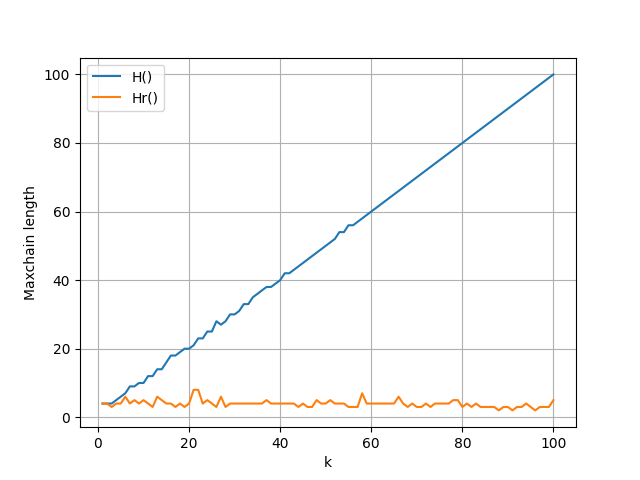
\includegraphics[scale=0.65]{plot5.png}
        	\caption{Graph of Maxchain length. \label{fig:1}}
        \end{figure}
        
        We see that the H() hashing function gives a linear line whereas the Hr() hashing function's max chain seems to be almost constant. This is because, as we increase k, the numbers in the set whose hashing table position is same increases linearly. Due to this, the max chain length too increases. But in the Hr() hashing function, the rx mod p part, helps "randomize" the number before applying the hashing function, thus reducing the max chain length and almost keeping it at a constant level.
\end{enumerate}

The code used to plot is pasted below:
\verbatiminput{4c.py}


%------------------------------------------------

\end{document}
